\documentclass[10pt,aspectratio=43]{beamer}

\usepackage{graphicx}
\graphicspath{{images/},{prebuilt_images/},{../../sharedimages/}}
\usepackage[sectionpages,
			rotationcw % clockwise, default is counterclockwise
			]{beamer}

\usepackage[utf8]{inputenc}
\usepackage[english]{babel}
\usepackage[T1]{fontenc}
\usepackage{csquotes}
\usepackage[titlenumbered,ruled,noend,english,onelanguage]{algorithm2e}

\SetKwFor{FOR}{For}{do}{end For}%

\usepackage[scaled]{beramono}
\usepackage[scale=1.05]{AlegreyaSans}
\usepackage{subcaption}
\usetikzlibrary{arrows.meta}
\usetikzlibrary{automata, positioning}
\usetikzlibrary{spy}
% \usepackage[backend=biber, citetracker=true, style=numeric]{biblatex}
% \addbibresource{../biblio/references_all.bib}


% Configure style for custom doubled line
\newcommand*{\doublerule}{\hrule width \hsize height 1pt \kern 0.5mm \hrule width \hsize height 2pt}

% Configure function to fill line with doubled line
\newcommand\doublerulefill{\leavevmode\leaders\vbox{\hrule width .1pt\kern1pt\hrule}\hfill\kern0pt }


\newcommand{\mytheorem}[2]{
\doublerulefill\ \framebox{\textbf{#1}}\ \doublerulefill
\vspace{0.1cm}

#2

\doublerulefill
}

\definecolor{javared}{rgb}{0.6,0,0} % for strings
\definecolor{javagreen}{rgb}{0.25,0.5,0.35} % comments
\definecolor{javapurple}{rgb}{0.5,0,0.35} % keywords
\definecolor{javadocblue}{rgb}{0.25,0.35,0.75} % javadoc
\definecolor{marron}{rgb}{0.64,0.16,0.16}
\definecolor{orange_js}{RGB}{230,159,0}

\newcommand{\mybold}[1]{\textcolor{marron}{\textbf{#1}}}
\newcommand{\cRm}[1]{\textsc{\romannumeral #1}}


%%%%%%%%%%%%%%%%%%%%%%%%%%%%%%%%%%%%%%%%%%%%%%%%%%%%%%%%%%%%%%%%%%%%%%%%%%%%%%%
%%%%%%%%%%%%%%%%%%%%%%%%%%%%%%%%%%%%%%%%%%%%%%%%%%%%%%%%%%%%%%%%%%%%%%%%%%%%%%%
% HEADER
%%%%%%%%%%%%%%%%%%%%%%%%%%%%%%%%%%%%%%%%%%%%%%%%%%%%%%%%%%%%%%%%%%%%%%%%%%%%%%%
%%%%%%%%%%%%%%%%%%%%%%%%%%%%%%%%%%%%%%%%%%%%%%%%%%%%%%%%%%%%%%%%%%%%%%%%%%%%%%%

\title[] %shown at the top of frames
{What is going on} %shown in title frame
\subtitle{}

\date{2021} % explicitly set date instead of \today

\author[]%shown at the top of frames
{%shown in title frame
	{Lefort Tanguy}%
}

\institute[
]
{% is placed on the bottom of the title page
    University of Montpellier
}


%%%%%%%%%%%%%%%%%%%%%%%%%%%%%%%%%%%%%%%%%%%%%%%%%%%%%%%%%%%%%%%%%%%%%%%%%%%%%%%
%%%%%%%%%%%%%%%%%%%%%%%%       PLAN      %%%%%%%%%%%%%%%%%%%%%%%%%%%%%%%%%%%%%%
%%%%%%%%%%%%%%%%%%%%%%%%%%%%%%%%%%%%%%%%%%%%%%%%%%%%%%%%%%%%%%%%%%%%%%%%%%%%%%%

\begin{document}
\maketitle

\begin{frame}{Our estimator}
Solve:
\[\min_{\substack{\beta \in \bbR^p \\ \Theta \in \bbR^q}}
\frac{1}{2 n} \norm{y - X\beta - Z\Theta}^2_2 +
\lambda_{\beta, \ell_1} \norm{\beta}_1 + \lambda_{\Theta, \ell_1} \norm{\Theta}_1 +
\frac{\lambda_{\beta, \ell_2}}{2} \norm{\beta}_2^2 + \frac{\lambda_{\Theta, \ell_2}}{2} \norm{\Theta}_2^2\enspace .\]
\begin{block}{CBPG solver operations}
    \[\beta^{k+1} =  \prox_{\frac{1}{L_X}g^{(1)}}\left(\beta^k - \frac{1}{L_X}\frac{\partial}{\partial \beta}f(\beta^k, \Theta^k)\right)\enspace,\]
    \[ \Theta^{k+1}_{\branch{q}{i}}= \prox_{\frac{1}{L_i}g^{(2)}}\left(\Theta^k_{\branch{q}{i}} - \frac{1}{L_i}\frac{\partial}{\partial \Theta_{\branch{q}{i}}}f(\beta^{k+1}, \Theta^k)\right)\]
\end{block}
\end{frame}

\begin{frame}{The issue of the eigenvalues}{Lanczos = power iteration with the power}
    \begin{itemize}
        \item We need the largest singular value of $Z_{\branch{q}{i}}^\top Z$ (upper bound with consistency),
        \item Power method too long for good values,
        \item Solution: use Lanczos iteration method.
    \end{itemize}
    \begin{algorithm}[H]
        \caption{Lanczos algorithm on an hermitian matrix H}
        \SetKwInOut{Input}{Input~}
        \SetKwInOut{Output}{Output~}
        \Input{$H\in \bbR^{n\times n}$, $m$ dimension of the Krylov subspace visited}

        $v_1$ random unit vector

        \FOR{$j=1,\dots,m-1$}{
            $ w_{j+1} = Hv_j$ \hspace{3cm} // visit a new direction \\
            $t_{k,j} = \langle v_k, w_{j+1} \rangle,\ k=1,\dots, j$ \\
            $w_{j+1} = w_{j+1} - \sum_{k=1}^j t_{k,j} v_k$  \hspace{.8cm} // orthogonalization\\
            $t_{j+1,j} = \|w_{j+1}\|$ \\
            $v_{j+1} = \frac{w_{j+1}}{t_{j+1, j}}$
        }
        \Output{$T$}
    \end{algorithm}
\end{frame}

\begin{frame}{Results with Lanczos}{We use Lanczow in our solvers}

\begin{figure}[!h]
	\begin{subfigure}{.4\paperwidth}
		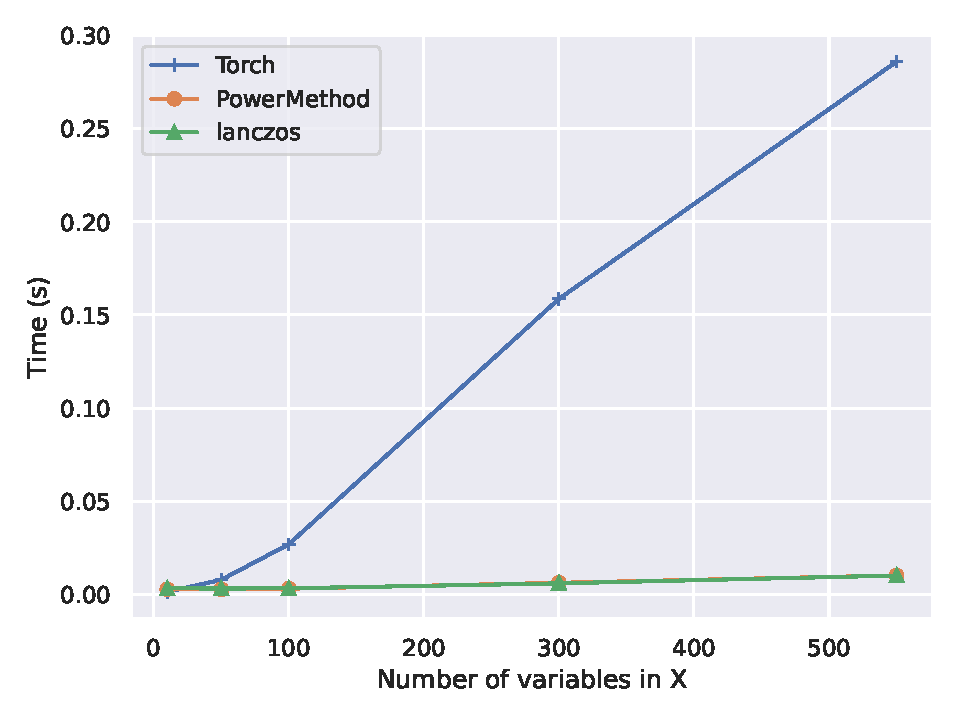
\includegraphics[width=\textwidth]{./prebuilt_images/benchmark_powermethod_scipy_n20000p550.pdf}
		\caption{Time to produce the result}
	\end{subfigure}
	\begin{subfigure}{.4\paperwidth}
		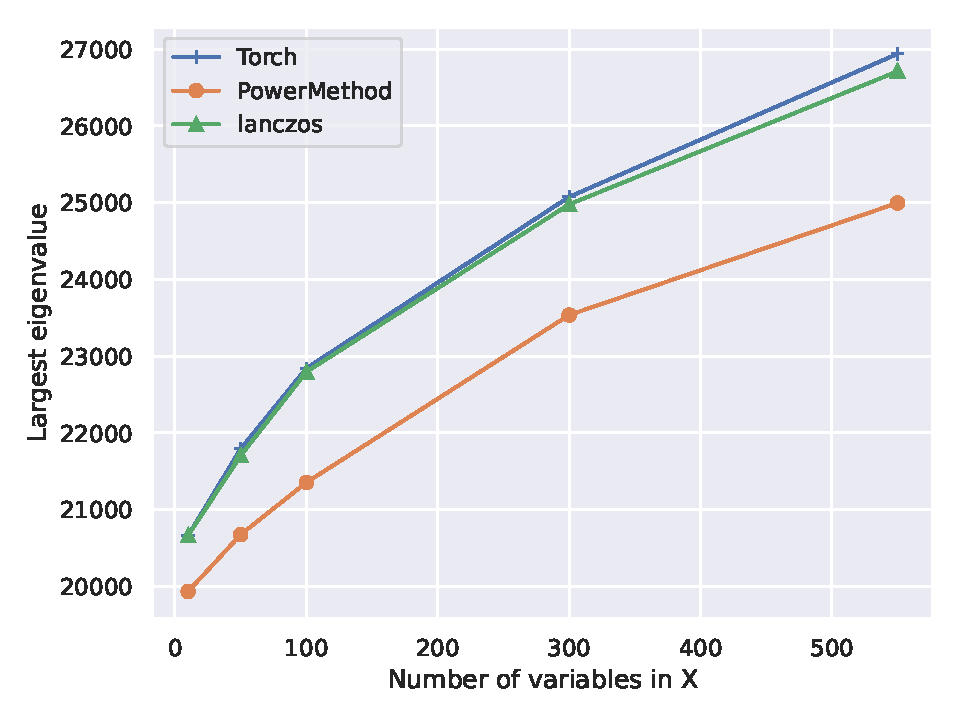
\includegraphics[width=\textwidth]{./prebuilt_images/benchmark_powermethod_scipy_values_n20000p550.pdf}
		\caption{Values of the largest singular value obtained.}
	\end{subfigure}
	\caption{Comparison of the linalg module of \texttt{Pytorch}, the power method and Lanczos algorithms to get the largest singular value of an hermitian matrix with $n=20000$ and a varying number of features up to $550$ }
	\label{fig:lanczos}
\end{figure}
\end{frame}


%%%%%%%%%%%%%%%%%%%%%%
% Sparsity
%%%%%%%%%%%%%%%%%%%%%%

\begin{frame}{Run on simulated data}{Because on genom data nothing converged...}
    \begin{figure}[ht!]
        \begin{subfigure}{.4\paperwidth}
            \centering
            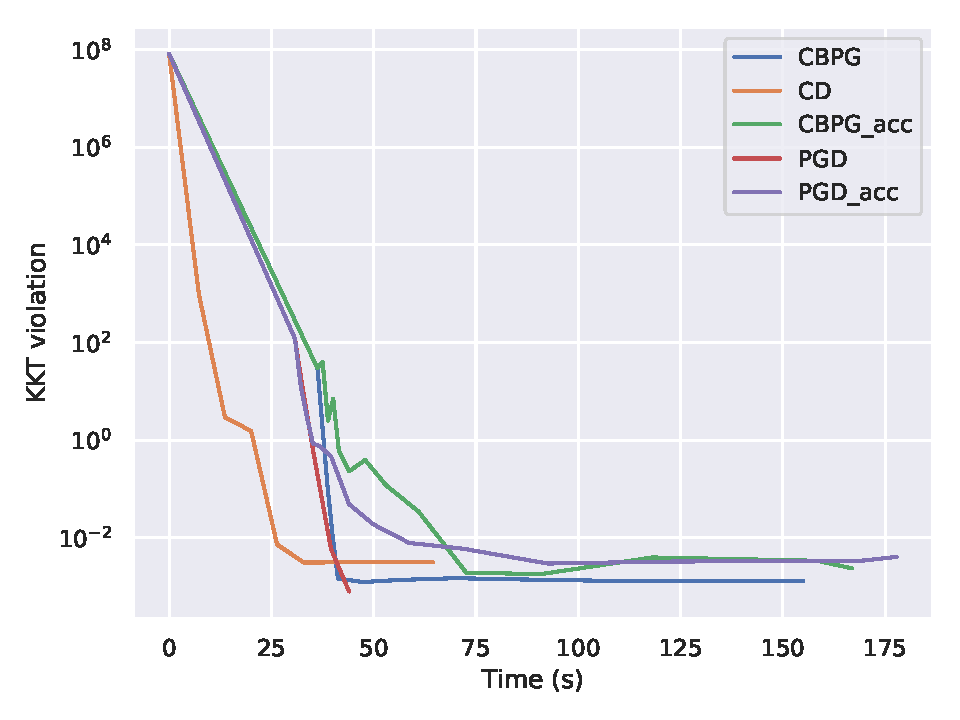
\includegraphics[width=\textwidth]{prebuilt_images/simulated_n20000p500_kkt_snr10.pdf}
            \caption{Regularizations are set to $\frac{\lambda_{\max}}{10}$.}
            \label{fig:simu_ccl}
        \end{subfigure}
        \begin{subfigure}{.4\paperwidth}
            \centering
            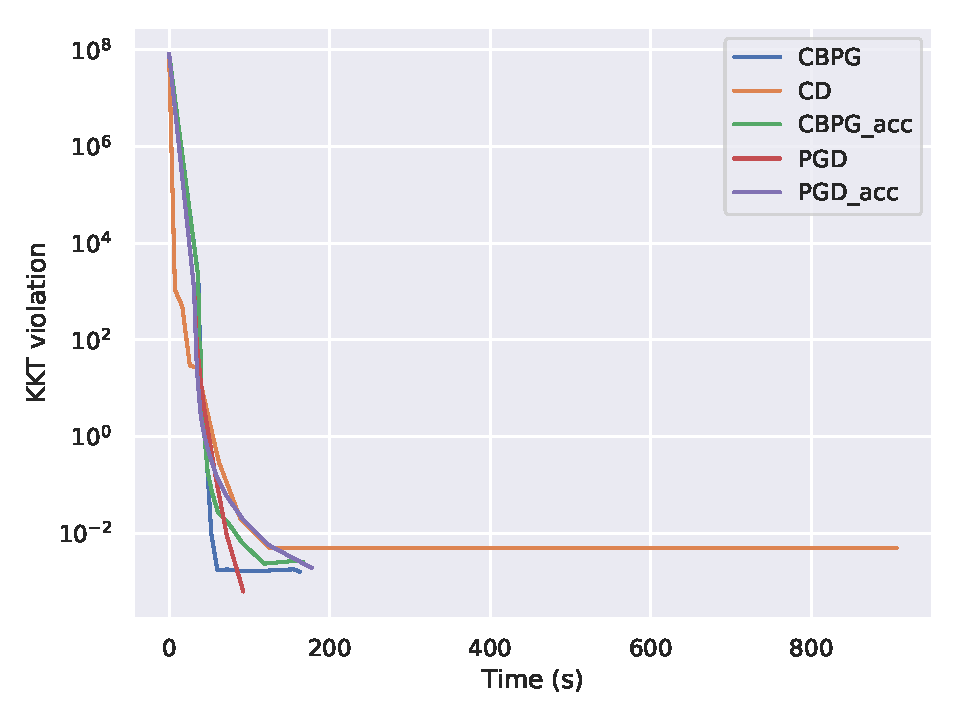
\includegraphics[width=\textwidth]{prebuilt_images/simulated_n20000p500_kkt_snr10_over100.pdf}
            \caption{Regularizations are set to $\frac{\lambda_{\max}}{100}$.}
            \label{fig:simu_ccl_over100}
        \end{subfigure}
        \caption{KKT criterion curves on the simulated regression dataset with $n=20000$ and $p=500$, $q=\frac{p(p+1)}{2}$.
        Maximum number of epochs is set to $100$. Float types are $32$-bytes. Sparsity level is $25\%$.
        }
    \end{figure}
    \begin{itemize}
        \item We're not better for every regularization, but are we where it matters?
    \end{itemize}
\end{frame}

\begin{frame}{When are the results the same sparsity?}
    \begin{figure}[ht]
        \centering
        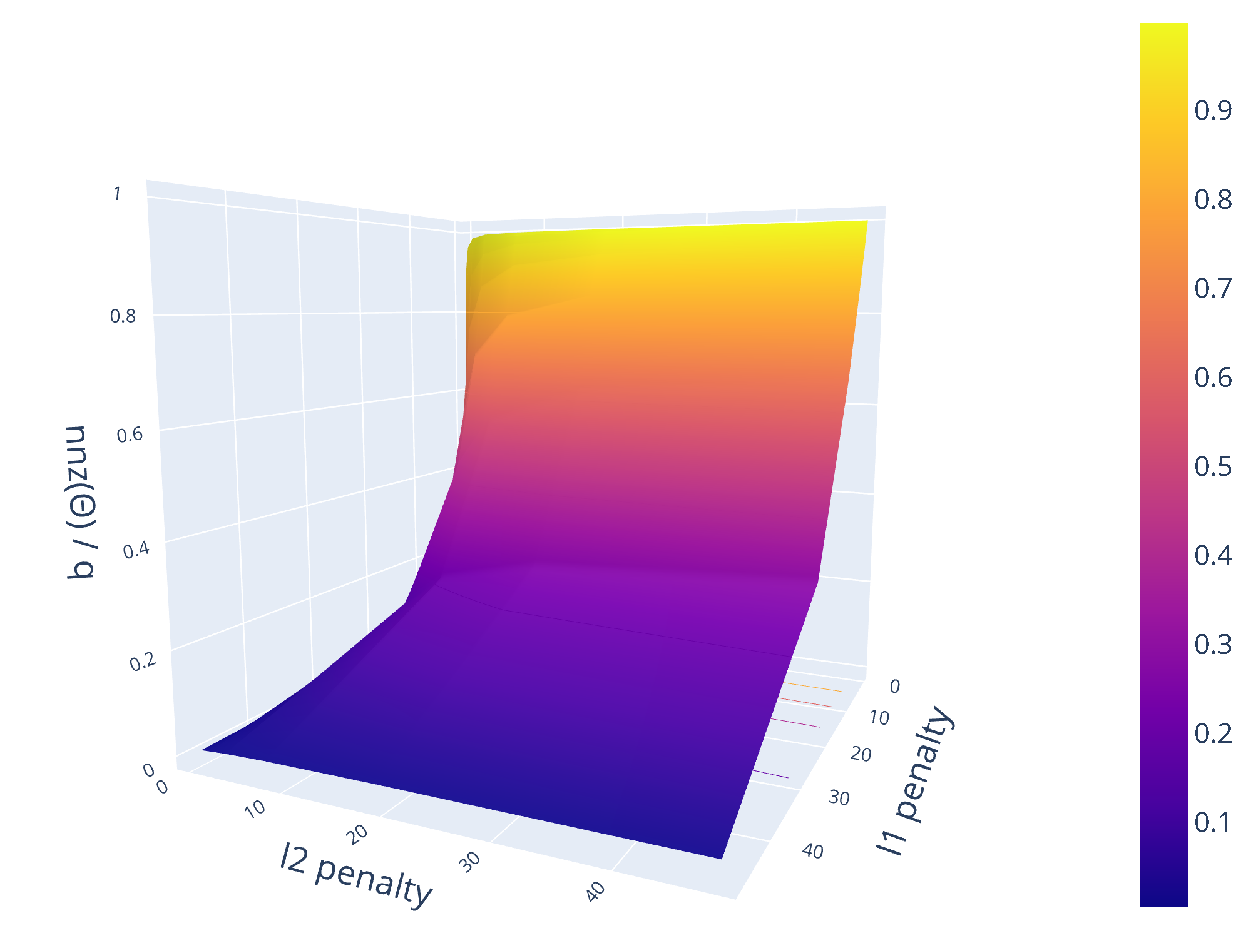
\includegraphics[scale=.3]{prebuilt_images/theta_surface_sparsity.pdf}
        \caption{Sparsity obtained in $\Theta$ with $n=20000$, $p=500$, $\mathrm{SNR}=10$, sparsity level simulated of $1\%$ in $\beta$ and $\Theta$, Float-$32$ types and $100$ epochs allowed.}
        \label{fig:sp_surf}
    \end{figure}

    \begin{itemize}
        \item BUT sparsity is not everything$\dots$ use a criterion like MSE
    \end{itemize}
\end{frame}

\begin{frame}{Look at paths instead of single runs}{Simulated $20000\times 500$ data}
In statistics we rarely only run one Elastic-Net,
    \begin{figure}[ht]
        \centering
        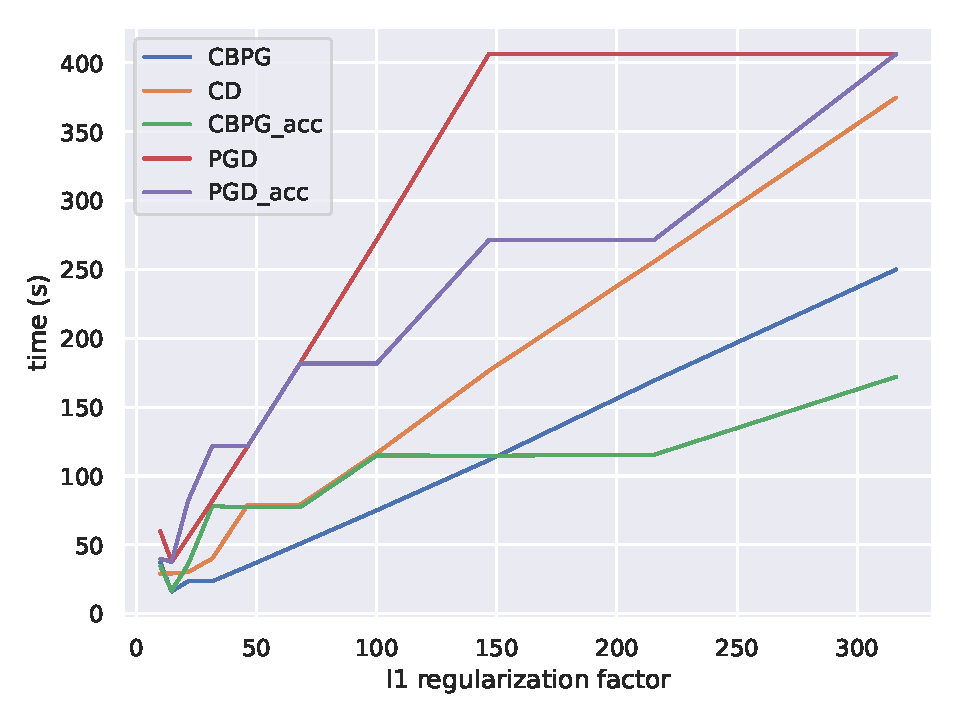
\includegraphics[scale=.35]{prebuilt_images/simu_total/simulated_n20000p500_snr=10_TIME_2605.pdf}
        \caption{SNR$=10$, $n=20000$, $=500$, $\Theta_i\in [-100, 100]$ and $\beta_i\in[-1000, 1000]$, $X_{ij}\sim\cN(0, 1)$, sparsity=$1\%$.}
    \end{figure}

    \begin{itemize}
        \item MSE of $\hat\beta - \beta^*$ and $\hat \Theta - \Theta^*$ consistant accross solvers, (graphs available)
        \item when CD is faster at the beginning, there isn't a large gain.
    \end{itemize}
\end{frame}

\begin{frame}{Can values in $\beta$ and $\Theta$ have an impact?}{On the search of an explanation for genom data}
    \begin{figure}
        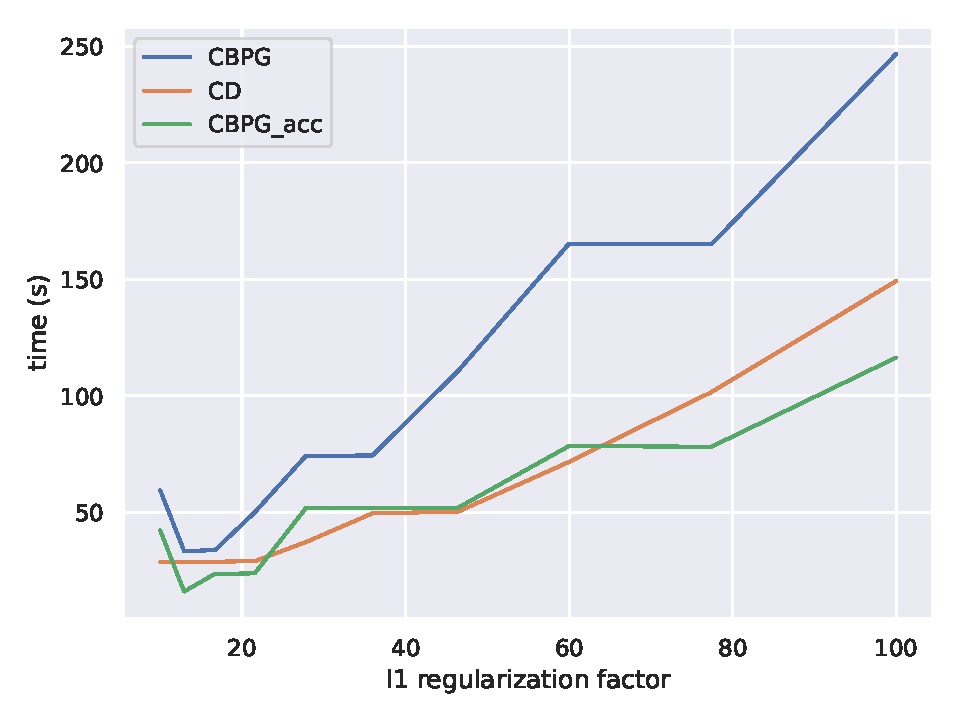
\includegraphics[scale=.35]{prebuilt_images/small_simu/simulated_n20000p500_snr=10_TIME_2705_beta100_theta_10.pdf}
        \caption{SNR$=10$, $n=20000$, $=500$, $\Theta_i\in [-10, 10]$ and $\beta_i\in[-100, 100]$, $X_{ij}\sim\cN(0, 1)$, sparsity=$1\%$.}
    \end{figure}

    \begin{itemize}
        \item It is harder for solvers to converge (but they all do, execpt PGD near the end so I removed it)
        \item the only real contender for beating CD is accelerated CBPG.
    \end{itemize}
\end{frame}


\begin{frame}{Let's talk about the genomic data then}{Why don't we converge easily?}
    The condition numbers for simulated data:
    \begin{itemize}
        \item on standardized $X$: $\kappa(X)\simeq 1.4$
        \item on standardized blocks: $\kappa(Z_{\branch{q}{i}}) < 2$
    \end{itemize}
    \pause
    But the genomic dataset isn't as well conditioned: $\kappa(X)\simeq 10^{14}$
    \begin{figure}
        \includegraphics[scale=.5]{prebuilt_images/condition_number_genom.pdf}
    \end{figure}
\end{frame}


\begin{frame}{Let's talk about the genomic data then}{Covariance matrix}
    \begin{figure}[ht!]
        \begin{subfigure}{.4\paperwidth}
            \centering
            \includegraphics[width=1.1\textwidth]{prebuilt_images/Gram_matrix_genom.pdf}
            \caption{Gram matrix of $X$.}
        \end{subfigure}
        \begin{subfigure}{.4\paperwidth}
            \centering
            \includegraphics[width=1.1\textwidth]{prebuilt_images/Gram_matrix_genom_60.pdf}
            \caption{Gram matrix of the $60$ first features.}
        \end{subfigure}
    \end{figure}
    \begin{alertblock}{Ill conditioned data}
        \begin{itemize}
            \item The first $60$ features are very ill conditioned,$\dots$
            \item but they are also the most important (nucleotide and dinucleotide levels).
        \end{itemize}
    \end{alertblock}
\end{frame}


\begin{frame}{Can we somehow precondition our data?}{Why not use what I learnt with logistic regression?}
    \begin{block}{ZCA whitening}
        \begin{itemize}
            \item What does it do? Transform $X$ st $\bbV(X)=\mathrm{I}d$
            \item How? $(X-\mu)W=Y$
            \item Problem: Many whitening possible (infinte number if we include rotations),
        \end{itemize}
    \end{block}
        \pause
        ZCA whitening chosen: minimize $\ell_2$ norm between before/after transformed data, symmetric ($\Sigma^{-1/2}$) and simple to compute.
        \medskip
        \begin{algorithm}[H]
            \caption{ZCA whitening of a centered matrix.}
            \SetKwInOut{Input}{Input~}
            \SetKwInOut{Output}{Output~}
            \Input{$X\in \bbR^{n\times p}$ with features means of $0$, $\epsilon >0$}

            $\Sigma = \frac{X^\top X}{n}$

            $U, \Lambda, V = \mathrm{SVD}(\Sigma)$ with $U\in\bbR^{p\times p}$ and $V\in\bbR^{n\times n}$


            $Y = X U (\Lambda + \epsilon\Id)^{-\frac{1}{2}} U^\top$

            \Output{$Y=XW^\top$}
        \end{algorithm}
\end{frame}

\begin{frame}{Condition number}{Covariance matrix}
    \begin{block}{Effect of the whitening}
        There is no miracle, very ill conditioned data can't become perfect.
        \begin{itemize}
            \item Diagonally dominant matrix (instead of identity) but close to identity nonetheless
        \end{itemize}
    \end{block}
    \begin{figure}[ht!]
        \begin{subfigure}{.4\paperwidth}
            \centering
            \includegraphics[width=1.1\textwidth]{prebuilt_images/Gram_matrix_genom_zca.pdf}
            \caption{Gram matrix of whitened $X$.}
        \end{subfigure}
        \begin{subfigure}{.4\paperwidth}
            \centering
            \includegraphics[width=1.1\textwidth]{prebuilt_images/Gram_matrix_genom_zca_60.pdf}
            \caption{Gram matrix of the $60$ first features whitened.}
        \end{subfigure}
    \end{figure}
    \end{frame}

\begin{frame}{Condition number}{Is there any interest of whitening?}
\begin{figure}
    \includegraphics[scale=.45]{prebuilt_images/condition_number_blocks_zca.pdf}
\end{figure}
\begin{block}{}
    \begin{itemize}
        \item $\kappa(X)=\cO(10^6)$
        \item Features are (almost) decorrelated (matrix made from train to avoid leakage),
        \item Features are also standardized in the process (when we divide by the eigenvalues).
    \end{itemize}
\end{block}
\end{frame}

\begin{frame}{Condition number}{Is there any interest of whitening?}
\begin{figure}
    \includegraphics[scale=.45]{prebuilt_images/condition_number_blocks_zca.pdf}
\end{figure}
\begin{block}{}
    \begin{itemize}
        \item $\kappa(X)=\cO(10^6)$
        \item Features are (almost) decorrelated (matrix made from train to avoid leakage),
        \item Features are also standardized in the process (when we divide by the eigenvalues).
    \end{itemize}
\end{block}
\end{frame}

\begin{frame}{Problem}{We change the preprocessing...}
    \begin{columns}
        \begin{column}{0.45\paperwidth}
            \centering
            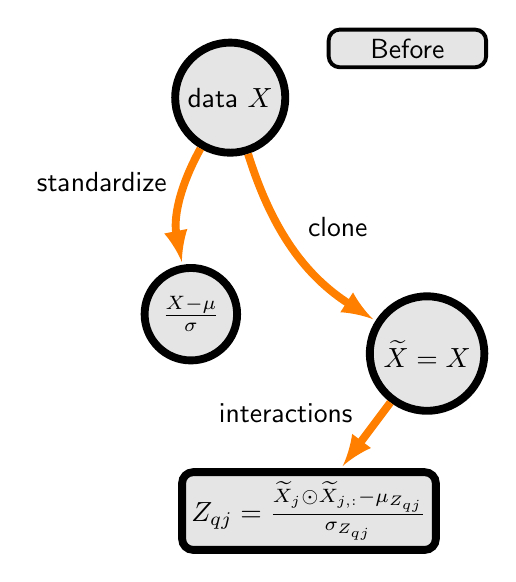
\begin{tikzpicture}[font=\sffamily, scale=0.5]

                % Setup the style for the states
                \tikzset{node style/.style={state,
                                            minimum width=1cm,
                                            line width=1mm,
                                            fill=gray!20!white,
                                            },
                        node time/.style = {shape   = rectangle,
                                            rounded corners,
                                            fill           = gray!20!white,
                                            minimum width  = 2cm,
                                            double = black,
                                            draw,
                                            align          = center,
                                            text           = black},
                        node Z/.style={state,
                                       shape = rectangle,
                                       rounded corners,
                                       minimum width=1cm,
                                       line width=1mm,
                                       fill=gray!20!white}}

                % Draw the states
                \node[node style] at (-0, 1.5)      (X)     {data $X$};
                \node[node style] at (-1, -4)      (std)     {$\frac{X-\mu}{\sigma}$};
                \node[node style] at (5, -5) (clone) {$\widetilde X = X$};
                \node[node Z] at (2, -9) (Z) {$Z_{\branch{q}{j}}=\frac{\widetilde X_j \odot \widetilde X_{\llbracket j,:\rrbracket} - \mu_{Z_{\branch{q}{j}}}}{\sigma_{Z_{\branch{q}{j}}}}$};
                \node[node time] at (4.5, 2.75)  (timer) {Before};

                % Connect the states with arrows
                \draw[every loop,
                      auto=right,
                      line width=1mm,
                      >=latex,
                      draw=orange,
                      fill=orange]
                    (X) edge[bend right=20] node {standardize} (std)
                    (X) edge[bend right=20, auto=left] node {clone} (clone)
                    (clone) edge node {interactions} (Z);
            \end{tikzpicture}
                \end{column}
                \vrule{}
        \begin{column}{0.45\paperwidth}
            \centering
            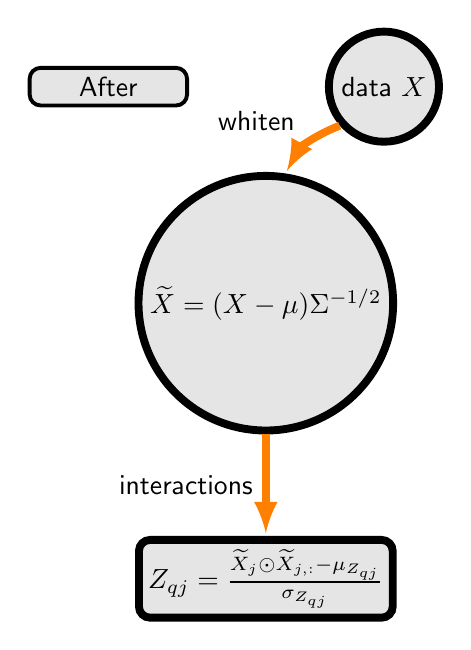
\begin{tikzpicture}[font=\sffamily, scale=0.5]

                % Setup the style for the states
                \tikzset{node style/.style={state,
                                            minimum width=1cm,
                                            line width=1mm,
                                            fill=gray!20!white,
                                            },
                        node time/.style = {shape   = rectangle,
                                            rounded corners,
                                            fill           = gray!20!white,
                                            minimum width  = 2cm,
                                            double = black,
                                            draw,
                                            align          = center,
                                            text           = black},
                        node Z/.style={state,
                                       shape = rectangle,
                                       rounded corners,
                                       minimum width=1cm,
                                       line width=1mm,
                                       fill=gray!20!white}}

                % Draw the states
                \node[node style] at (7, 1.5)  (X)   {data $X$};
                \node[node style] at (4, -4) (whiten) {$\widetilde X = (X-\mu)\Sigma^{-1/2}$};
                \node[node Z] at (4, -11) (Z) {$Z_{\branch{q}{j}}=\frac{\widetilde X_j \odot \widetilde X_{\llbracket j,:\rrbracket} - \mu_{Z_{\branch{q}{j}}}}{\sigma_{Z_{\branch{q}{j}}}}$};
                \node[node time] at (0, 1.5)  (timer) {After};

                % Connect the states with arrows
                \draw[every loop,
                      auto=right,
                      line width=1mm,
                      >=latex,
                      draw=orange,
                      fill=orange]
                    (X) edge[bend right=20] node {whiten} (whiten)
                    (whiten) edge node {interactions} (Z);
            \end{tikzpicture}
        \end{column}
        \end{columns}
\end{frame}

\begin{frame}{Another problem}{...}
\begin{alertblock}{Time speed up}
There is a new hyperparameter to tune!
\end{alertblock}
\end{frame}

\begin{frame}{NEW DEVELOPMENT}{(not ZCA related yet)}

    \begin{itemize}
        \item I was working with $\ell_2$ penalties $\simeq \lambda_{\max} / 5$ (or $2$ or $10$),
        \item Using $\times 2$ or $\times 5$ did not really fasten (or at least the number of epochs needed was very high so I didn't see it)
        \item Why not recompute the residuals every $100$ epochs
        \item Why not put a very high $\ell_2$ penalty as the data is very ill conditioned ($_times 50$)? (useful in practice?)
    \end{itemize}

    \begin{figure}[ht!]
        \begin{subfigure}{.4\paperwidth}
            \centering
            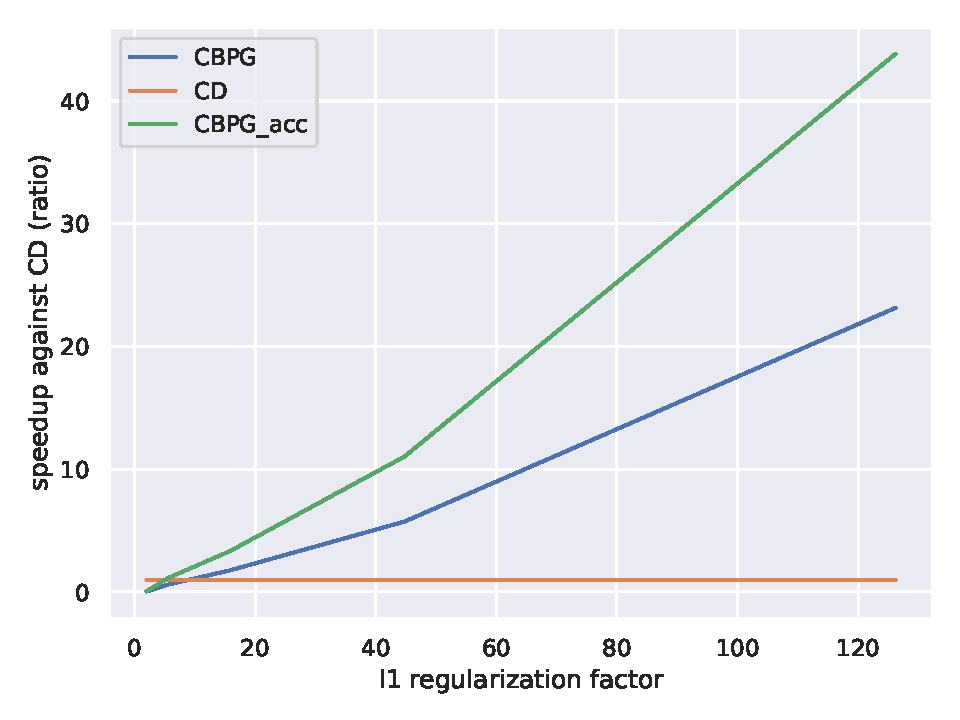
\includegraphics[width=1.1\textwidth]{prebuilt_images/genom/genom_bigl2_ratio.pdf}
            \caption{Time ratio of speed up against CD.}
        \end{subfigure}
        \begin{subfigure}{.4\paperwidth}
            \centering
            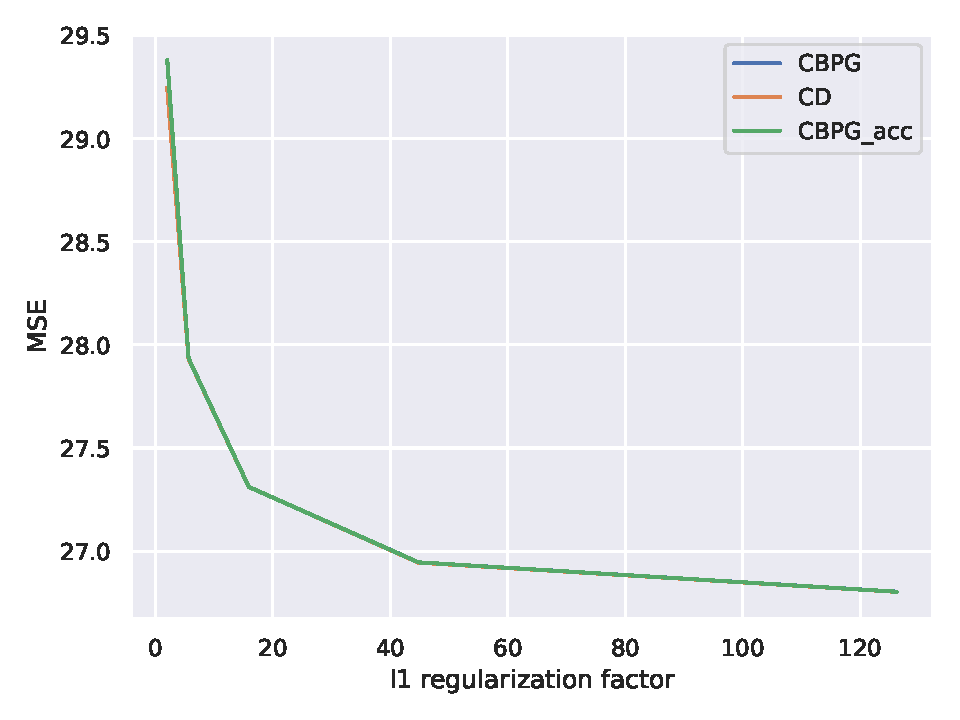
\includegraphics[width=1.1\textwidth]{prebuilt_images/genom/genom_bigl2_MSE.pdf}
            \caption{Results are consistent accross solvers and MSE is good (need to go further in the PATH).}
        \end{subfigure}
    \end{figure}
\end{frame}

\begin{frame}{TODO}
    TODO for experiments:
    \begin{itemize}
        \item Try with ZCA and several values of $\epsilon$
        \item Is it realistic such $\ell_2$ penalty? (try lower and see the MSE for sure)
        \item If ZCA is good, what features does it select?
        \item Are they the same as without ZCA albeit the interactions are built the same anymore?
    \end{itemize}
\pause
    TODO for report:
    \begin{itemize}
        \item Redo the matvec products benchmarks without KeOps to legitimize that computing KKT violition is really not costly at all even if $\cO(np+nq)$
        \item Talk more about multicolinearity that legitimizes the enet
        \item Explain what is a GPU and how does it work (drawings will be needed + Benjamin)
        \item ToSee
    \end{itemize}
\end{frame}
\end{document}